\documentclass[11pt]{article}
\usepackage[a4paper,margin=22mm,headheight=16pt]{geometry}
\usepackage{fontspec,xeCJK,xcolor,graphicx,enumitem,fancyhdr,titlesec}
\usepackage{hyperref}
\IfFontExistsTF{Times New Roman}{\setmainfont{Times New Roman}}{\setmainfont{TeX Gyre Termes}}
\IfFontExistsTF{FangSong}{\setCJKmainfont[AutoFakeBold=2]{FangSong}}{\IfFontExistsTF{仿宋}{\setCJKmainfont[AutoFakeBold=2]{仿宋}}{\IfFontExistsTF{FandolFang-Regular.otf}{\setCJKmainfont[AutoFakeBold=2]{FandolFang-Regular.otf}}{\setCJKmainfont{FandolSong-Regular.otf}}}}
\definecolor{ink}{HTML}{173747}\definecolor{accent}{HTML}{227E82}
\hypersetup{colorlinks=true,urlcolor=accent,linkcolor=accent}
\linespread{1.22}\setlength{\parindent}{0pt}\setlength{\parskip}{6pt}
\setlist[itemize]{leftmargin=1.4em,itemsep=3pt}
\titleformat{\section}{\large\bfseries\color{ink}}{}{0pt}{}
\titlespacing*{\section}{0pt}{14pt}{7pt}
\pagestyle{fancy}\fancyhf{}\lhead{\small OMNI LEARNING / 学习手册}\rhead{\small Source-grounded learning}\cfoot{\small\thepage}
\emergencystretch=2em\widowpenalty=10000\clubpenalty=10000
\newcommand{\Needspace}[1]{\par\begingroup\dimen0=#1\relax\vskip0pt plus\dimen0\penalty-100\vskip0pt plus-\dimen0\vskip\dimen0\penalty9999\vskip-\dimen0\vskip0pt\endgroup}
\begin{document}


{\LARGE\bfseries\color{ink} 价格如何协调供需}\par

2026-10-08 | Day02/30 | 阅读 8 分钟 + 练习 3 分钟\par\vspace{6pt}

\Needspace{5\baselineskip}\section*{今日导航}

今天回答：面包涨价一定说明大家更爱吃面包了吗？目标是区分需求、供给与价格变化，并避免只凭价格推断原因。先回忆昨日机会成本：面包价格提高时，消费者放弃其他消费的代价如何变化？

\Needspace{5\baselineskip}\section*{先把市场的两边分开}

买方在不同价格下愿意且能够购买多少，构成需求关系；卖方在不同价格下愿意且能够出售多少，构成供给关系。基础模型通常先保持其他条件不变，再观察价格与数量。[S4] 图 B 同时画买方和卖方，是提醒我们：价格由双方互动形成，不能只从一边的情绪解释。排队的图像本身也不足以证明短缺。

\begin{center}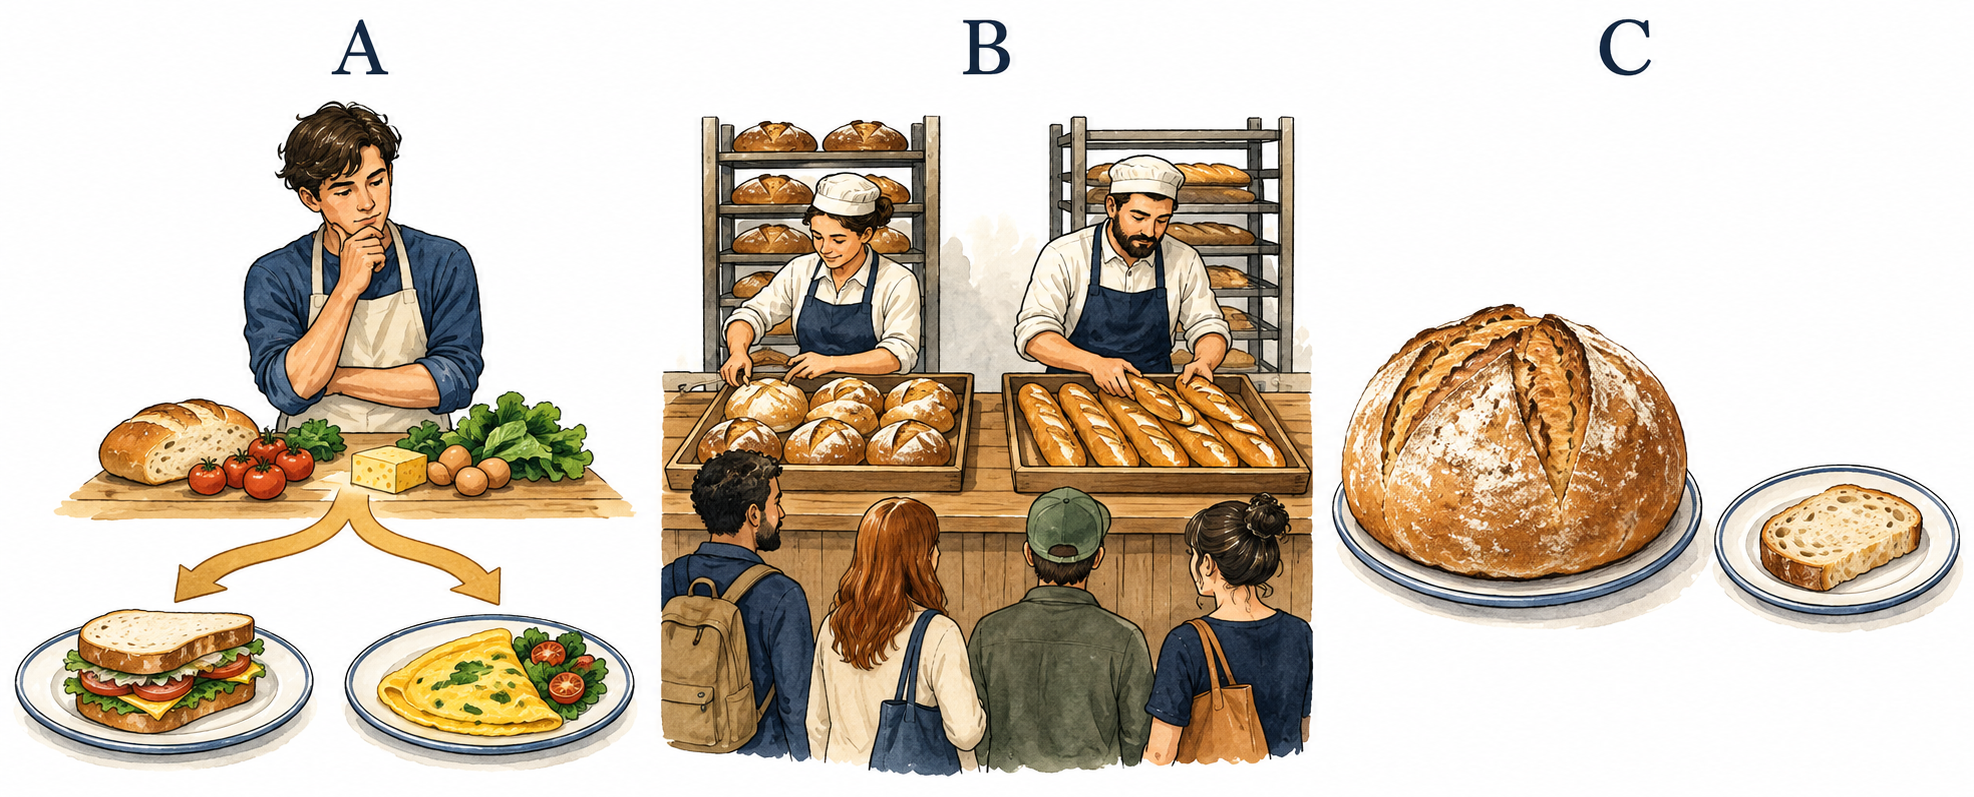
\includegraphics[width=\linewidth,height=0.26\textheight,keepaspectratio]{../assets/figure-a92b6089a95f.png}\par

{\small 本课重点看 B 区。A 同一组资源对应不同选择；B 买方与卖方共同形成市场；C 整体收益与额外一单位收益要分开计算。}\par

{\footnotesize AI生成教学示意，非实物照片、原始史料或官方架构。生成方式：内置文生图；提示词见仓库 docs/image-prompts.json。}\end{center}

\Needspace{5\baselineskip}\section*{沿曲线移动与曲线移动}

如果其他条件不变，只是面包自身价格变化，我们讨论的是需求量或供给量沿原关系变化。若消费者人数增加、偏好变化，或者面粉与能源成本变化，原来的关系可能整体改变。[S5]

“需求增加”与“涨价后少买”描述不同变化。前者是在相同价格下想买得更多，后者是价格变化引起的购买量调整。区分这两个说法，能避免把结果写成原因。在真实市场中，多个因素常同时变化，简化模型主要帮助提出问题，不保证只凭两条曲线就能预测一切。

\Needspace{5\baselineskip}\section*{两种涨价故事}

教学情形甲：面包店周边新开办公楼，午餐客流增加，生产条件暂时不变。需求上升可能推动价格与交易量同时上升。情形乙：原料变贵，消费者习惯不变，供给受影响可能推动价格上升而交易量下降。

两种情况下都可能看到涨价，但数量方向不同，原因也不同。观察到“价格涨、数量增”仍不是需求变化的最终证明，因为供给也可能同时变化。你至少需要比较时间段、产品是否相同、成本和客流等证据。均衡只表示模型内买卖数量相匹配，不代表结果必然公平，也不代表每个人都满意。[S4]

\Needspace{5\baselineskip}\section*{三分钟练习与自查}

把以下变化分别归为“需求条件”“供给条件”或“该商品自身价格”：面粉涨价；附近人口增加；这家店把同款面包标价调高。再为前两项各写一个需要核实的数据。

参考：面粉属于供给成本，需要采购账单或原料价格；人口属于潜在需求条件，需要实际客流或购买数据；店内标价是商品自身价格。不要把“人口增加”直接等同于“实际需求一定增加”，新增人口也可能不购买这类面包。

\Needspace{5\baselineskip}\section*{复盘与明日连接}

先分清哪一边的条件变了，再看价格和数量怎样共同变化。对新闻中的“涨价因为需求旺盛”，可以追问还有哪些供给证据。明天回到个人和企业的具体决策：是否继续多做一点，应看总收益还是额外收益？

\Needspace{6\baselineskip}\section*{扩展学习 / Further reading}\small 以下为选读，不计入每日必做时间。\begin{enumerate}[leftmargin=1.6em]

\item [S1] \href{https://openstax.org/books/principles-economics-3e/pages/1-1-what-is-economics-and-why-is-it-important}{What Is Economics, and Why Is It Important?} — 从稀缺与分工建立课程起点；文中旧统计不作为现状。\par OpenStax | 发布：未标注 | 核验：2026-10-08

\item [S2] \href{https://openstax.org/books/principles-economics-3e/pages/2-1-how-individuals-make-choices-based-on-their-budget-constraint}{Budget Constraint and Individual Choices} — 重点读机会成本、预算约束与边际分析。\par OpenStax | 发布：未标注 | 核验：2026-10-08

\item [S3] \href{https://openstax.org/books/principles-economics-3e/pages/2-2-the-production-possibilities-frontier-and-social-choices}{Production Possibilities Frontier} — 把个人选择扩展为社会资源配置，观察模型假设。\par OpenStax | 发布：未标注 | 核验：2026-10-08

\item [S4] \href{https://openstax.org/books/principles-economics-3e/pages/3-1-demand-supply-and-equilibrium-in-markets-for-goods-and-services}{Demand, Supply, and Equilibrium} — 对照需求、供给和均衡的图形定义。\par OpenStax | 发布：未标注 | 核验：2026-10-08

\item [S5] \href{https://openstax.org/books/principles-economics-3e/pages/3-2-shifts-in-demand-and-supply-for-goods-and-services}{Shifts in Demand and Supply} — 区分价格变化引起的沿曲线移动与其他条件变化引起的曲线移动。\par OpenStax | 发布：未标注 | 核验：2026-10-08

\end{enumerate}

\end{document}